\chapter{度量指标}
在机器学习、数据挖掘、推荐算法等学术实验分析阶段,通常要经过一个模型性能评价的过程。
%模型评价依赖于两方面因素:评价指标与公开数据集。
本章主要介绍在各个领域常用的评价或度量指标。
%公开数据集、数据采样技术、数据标准化和交叉检验。

\ornamento

%度量空间(Metric Space)和测度(Measure Theory in Probability)
\section{度量空间与测度论}
\section{范数}
\subsection{H\"{o}lder范数}
对于无约束范数逼近问题:
\begin{equation}\label{eq:normmin}
    \min~\|Ax - b\|_p
\end{equation}
其中,$A\in \mathbb{R}^{m\times n}, b\in \mathbb{R}^m$,$p>0$。

如果$p\ge 2$,则范数是$\ell_p$范数或称H\"{o}lder范数:
\begin{equation}
    f(x) \triangleq \|Ax - b\|_p = \Big[\sum\limits_i |a_i^T x - b_i|^p\Big]^\frac{1}{p}.
\end{equation}

我们定义
\[
    g(x) \triangleq f(x)^p = \|Ax - b\|_p^p = \sum\limits_i |a_i^T x - b_i|^p
\]
由于$g(x)$二阶处处可微,根据Newton法,可以得到下面的迭代序列:
\begin{equation}
    \begin{array}{lll}
      x_{k+1} & = & x_k -\alpha_k (\nabla^2 g(x_k))^{-1} \nabla g(x_k) \\
       & = & x_k - \frac{\alpha_k}{p-1} (A^T W_k A)^{-1} A^T W_k (A x_k - b) \\
       & = & \frac{p - 1 - \alpha_k}{p-1} x_k + \frac{\alpha_k}{p-1} (A^T W_k A)^{-1} A^T W_k b \\
       & = & \frac{p - 1 - \alpha_k}{p-1} x_k + \frac{\alpha_k}{p-1} \argmin\limits_{\bar{\omega}} \|W_k^{1/2}(A \bar{\omega} - b)\|_2
    \end{array}
\end{equation}
其中,$x_0 = 0$,$\alpha_k\in [0,1)$是固定的,或者根据线性搜索技术迭代变化。$W_k$是个对角矩阵:
\begin{equation}
    W_k \triangleq
    \begin{pmatrix}
        (a_1^T x_k - b_1)^{p-2} & 0 & \cdots & 0 \\
        0 & (a_2^T x_k - b_2)^{p-2} & \cdots & 0 \\
        \vdots & \vdots & \ddots & \vdots \\
        0 & 0 & 0 & (a_m^T x_k - b_m)^{p-2}
    \end{pmatrix}
\end{equation}

\subsection{曼哈顿范数}
当$p=1$时,问题\eqref{eq:normmin}转化为最小化$\ell_1$或曼哈顿范数(Manhattan Norm):
\[
    f(x) \triangleq \|Ax - b\|_1 = \sum\limits_i |a_i^T x - b_i|
\]
我们可以藉由下面的线性规划问题进行求解:
\[
    \begin{array}{ll}
      \textit{min} & \sum\limits_i \nu_i \\
      \textit{s.t.} & |a_i^T x - b_i|\le \nu_i, i = 1,\ldots,m \\
    \end{array}
\]

在机器学习任务中,常涉及到稀疏模型的训练问题,通过优化$\ell_1$正则项的非平滑损失函数学习模型,比如回归分析中的Lasso算法。

\subsection{欧式范数}
当$p=2$时,问题\eqref{eq:normmin}就是$\ell_2$或者欧式范数(Euclidean Norm)的最小化:
\[
    f(x) \triangleq \|Ax - b\|_2 = \sqrt{\sum\limits_i (a_i^T x - b_i)^2}
\]
是典型的最小二乘问题,存在下面等价的二次规划形式:
\[
    \min~f(x)^2 = \|Ax - b\|_2^2 = \sum\limits_i (a_i^T x - b_i)^2
\]
存在解析解(Analytic Solution, Closed Form Solution)
\[
    \hat x = (A^T A)^{-1}A^T b
\]

\subsection{切比雪夫范数}
当$p = \infty$时,问题\eqref{eq:normmin}转化为最小化$\ell_{\infty}$或者切比雪夫范数(Chebyshev Norm,也称“棋盘距离”):
\[
    f(x) \triangleq \|Ax - b\|_{\infty} = \max\limits_i |a_i^T x - b_i|
\]
由于不存在解析解,我们可以将其转化为下面的线性规划问题:
\[
    \begin{array}{ll}
      \textit{min} & \nu \\
      \textit{s.t.} & |a_i^T x - b_i|\le \nu, i = 1,\ldots,m \\
    \end{array}
\]

\subsection{L最大范数}
向量$\omega\in \mathbb{R}^m$的\textbf{L最大范数(Largest-L Norm)}$\|\omega\|_{[L]}$是将$\omega$按照其坐标绝对值降序排列,前$L$个最大坐标绝对值之和,即有定义
\begin{equation}\label{eq:largestlnorm}
    \|\omega\|_{[L]} = \sum\limits_{i=1}^L |\omega|_{[i]}, ~~~1\le L\le m,
\end{equation}
其中,$|\omega|_{[i]}$表示坐标绝对值降序排列第$i$位的数值,满足$|\omega|_{[1]} \ge |\omega|_{[2]} \ge \ldots \ge |\omega|_{[m]}$。
当$L=1$时,L最大范数等价于$\ell_{\infty}$范数;当$L=m$时,等价于$\ell_1$范数;当$1 < L < m$时,它是一个凸函数,最小化L最大范数等价于解线性规划问题
\begin{equation}\label{eq:minlargestlnorm}
    \begin{array}{ll}
      \textit{min} & \sum\limits_i c_i + Lq \\
      \textit{s.t.} & |a_i^T x - b_i|\le c_i + q,\\
      & c_i \ge 0, ~~~1\le i\le m.
    \end{array}
\end{equation}
多数人在面对最小化L最大范数问题时,会选择复杂的障碍函数法(Barrier Method)或次梯度法(Subgradient Method),纵然是优化问题专业人员亦鲜有人知可使用模型\eqref{eq:minlargestlnorm}简化问题。

\section{距离和相似性度量}
距离度量衡量对象间的差异程度,距离越远则对象间的差异越大。相似度度量衡量对象间的相似程度,与距离度量相反,相似度度量值越小,则说明对象间相似度越小,差异越大。其他相似性度量、距离度量可以参考\cite{cha2007comprehensive,lenz2008proximities}。

\subsection{闵可夫斯基距离}
闵可夫斯基距离(Minkowski Distance)是对多个距离度量公式的概括性的表述,公式如下:
\begin{equation}\label{eq:minkowski}
    d(x,y)=\Big[\sum\limits_i (x_i-y_i)^p\Big]^\frac{1}{p}
\end{equation}

\begin{enumerate}
  \item 当$p=1$时,闵可夫斯基距离退化成曼哈顿距离(Manhattan Distance):
      \begin{equation}\label{eq:manhattan}
        d(x,y) = \sum_i |x_i-y_i|
      \end{equation}
  它来源于城市区块距离,对多个维度上的距离求和。假设在曼哈顿街区乘坐出租车从一个地方到另一个地方,白色区域表示高楼大厦,灰色表示街道,三条折线都表示两地间的曼哈顿距离,三者长度相等。
  \begin{figure}[htbp]
    \centering
    \includegraphics[width=0.5\textwidth, height=6cm]{figures/ManhattanBlock.eps}\\
    \caption{曼哈顿街区与曼哈顿距离}\label{fig:manhattanblock}
  \end{figure}
  \item 当$p=2$时,闵可夫斯基距离退化成欧几里得距离(Euclidean Distance):
      \begin{equation}\label{eq:euclidean}
        d(x,y)=\sqrt {\sum\limits_i (x_i-y_i)^2}
      \end{equation}
  它是最常见的距离度量,衡量的是多维空间中点与点之间的绝对距离。如图~\ref{fig:manhattanblock}所示,中间绿色斜线表示两地之间的欧几里得距离。
  \item 当$p\rightarrow \infty$时,闵可夫斯基距离退化为切比雪夫距离(Chebyshev Distance):
      \begin{equation}\label{eq:chebyshev}
        d(x,y)=\lim_{p \rightarrow \infty}\Big[\sum\limits_i (x_i-y_i)^p\Big]^{1/p}=\max_{i} |x_i-y_i|
      \end{equation}
  它起源于国际象棋规则下国王的走法。
\end{enumerate}
  \begin{figure}[htbp]
    \centering
    \includegraphics[width=0.9\textwidth, height=1cm]{figures/UnitMinkowskiDist.eps}\\
    \caption{参数$p$与单位闵科夫斯基距离之间的关系图}\label{fig:unitminkowski}
  \end{figure}

\subsection{Cayley距离}
Cayley距离是度量有序变量无序性的指标。假设标准队列为$a$,$b$中至少有一个位置与$a$不同,通过交换$b$中的元素的位置可以将其变成标准队列(简称标准交换),Cayley距离对应最小的标准交换次数。如图\ref{fig:cayleydist},第一个队列是标准队列,我们可以最少交换三次第二个队列的位置对就可以变成标准队列,因此二者的Cayley距离为3。

\subsection{Ulam距离}
Ulam距离与Cayley距离类似,针对队列$b$,它可以使用删除-移动-插入的连环动作变成标准队列(简称标准变换)。Ulam距离对应最小的标准变换次数。如图
\ref{fig:ulamdist},第一个队列是标准队列,我们可以最少交换三次第二个队列的位置对就可以变成标准队列,因此二者的Ulam距离为2。

\begin{figure}[htbp]
    \begin{minipage}[t]{0.49\linewidth}
        \centering
          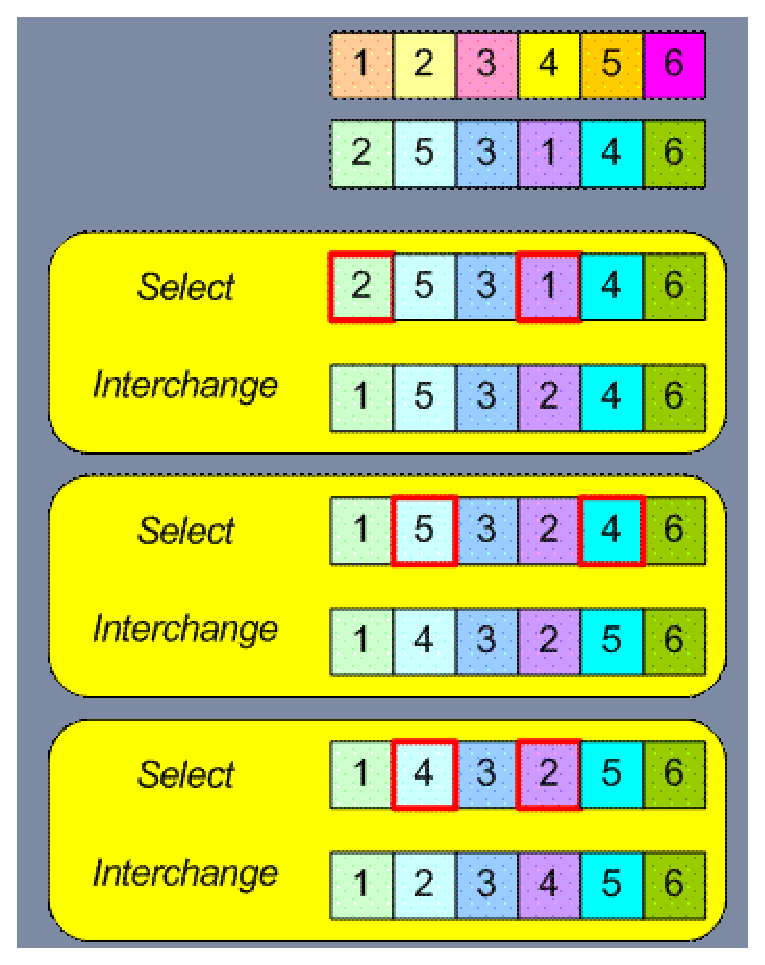
\includegraphics[width=0.95\textwidth,height=8cm]{figures/cayleydist}
          \caption{Cayley距离距离演示}\label{fig:cayleydist}
    \end{minipage}
    \begin{minipage}[t]{0.49\linewidth}
        \centering
          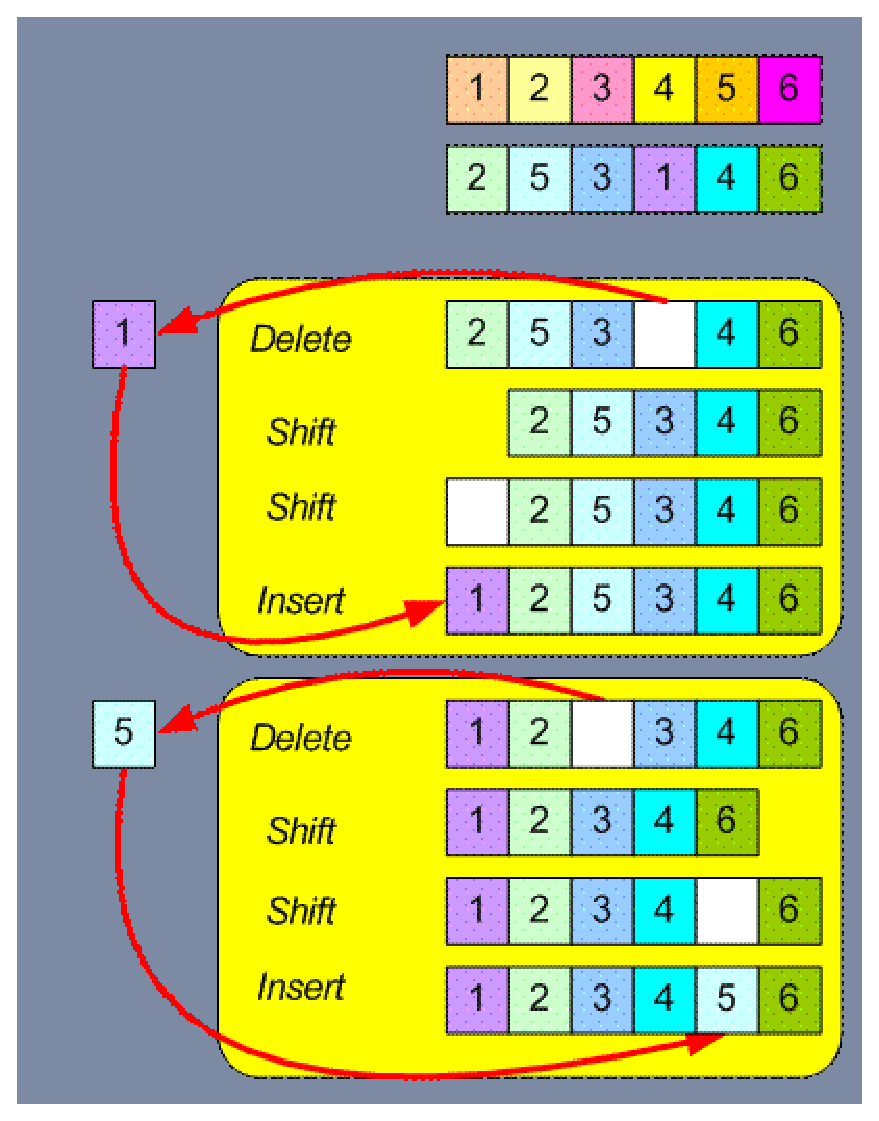
\includegraphics[width=0.95\textwidth,height=8cm]{figures/ulamdist}
          \caption{Ulam距离计算演示}\label{fig:ulamdist}
    \end{minipage}
\end{figure}

\subsection{汉明距离}
1950年,Richard Hamming~\cite{hamming1950error}引入了汉明距离(Hamming distance),亦称“信号距离”,用于度量两个等长字串相应位置字符不同的位置数目。汉明 距离还可以表示将一个字串变成另外一个字串需要替换的最小数目。对于两个二元字串$a,b$,它们的汉明距离即$a$ \textit{XOR} $b$中1的数目。

\subsection{月球漫步者距离}
它由Gaspard Monge在1781年首次提出,用以度量两个统计分布的差异。在数学上又称Wasserstein度量。

\subsection{余弦相似度}
向量空间两个向量夹角余弦值常用于衡量对象间的差异,具体定义如下:
\begin{equation}\label{eq:cosinesim}
    \cos\langle x,y\rangle=\frac{x^T y}{\|x\|\|y\|},
\end{equation}
余弦值越大,则两对象之间的差异越小;反之,则越大。余弦值可以直接用于度量对象之间的相似程度,此时称作\textbf{余弦相似度}(cosine similarity)。

\subsection{杰卡德系数}
对于两个集合$A$和$B$,如果我们只关心两者具有相同特征的比例,则可以使用如下形式的杰卡德系数(Jaccard coefficient)
\begin{equation}\label{eq:jaccard}
    J(A,B)=\frac{|A\cap B|}{|A\cup B|}
\end{equation}
度量对象间的相似程度。系数值越大,表明两个对象的相似性越强,反之则越弱。

\subsection{核相似度}
在实际应用中,我们可以直接将定义在向量空间上的核函数作为相似性度量,从而可以得到核相似性度量(kernel similarity)。比如高斯核函数定义的高斯相似性度量:
\begin{equation}\label{eq:kernelsim}
    K(x,y)=\exp\{-\frac{\|x-y\|^2}{2\sigma^2}\}.
\end{equation}

\subsection{皮尔逊相关系数}
皮尔逊相关系数(Pearson correlation coefficient)描述了两个变量间的线性相关性。对于变量$x$和$y$,假设均值分别是$\mu_x,\mu_y$,标准差分别是$\sigma_x,\sigma_y$,则总体相关系数定义如下:
\begin{equation}\label{eq:pearsoncor}
    \rho(x,y)=\frac{\cov(x,y)}{\sigma_x\sigma_y}=\frac{E\big[(x-\mu_x)(y-\mu_y)\big]}{\sigma_x\sigma_y}.
\end{equation}
基于$n$组样本对协方差和标准差的估计,我们可以使用下式计算样本相关系数:
\begin{equation}\label{eq:pearsonrho}
    \rho(x,y)=\frac{\sum\limits_i (x_i - \bar x)(y_i - \bar y)}{\sqrt{\sum\limits_i (x_i - \bar x)^2 \sum\limits_i (y_i - \bar y)^2}} = \frac{n\sum\limits_i (x_i y_i) - \sum\limits_i x_i \sum\limits_i y_i}{\sqrt{n\sum\limits_i x_i^2 - (\sum\limits_i x_i)^2}\sqrt{n\sum\limits_i y_i^2 - (\sum\limits_i y_i)^2}}.
\end{equation}
根据定义,皮尔逊相关系数$-1 \le \rho(x,y) \le 1$,通过$|\rho(x,y)|$的大小可以判定相关程度,$|\rho(x,y)|$越大,$x$和$y$的相关程度越大。当$\rho(x,y)=1$ 时,表示$x$和$y$完全正相关;当$\rho(x,y)=-1$表示完全负相关;当$\rho(x,y)=0$表示不相关。如果我们令$u_i=x_i-\bar x$,$v_i=y_i-\bar y$,$i=1,2,\ldots,n$,则皮尔逊相关系数实际上与夹角余弦相似度等价:
\begin{equation}
    \rho(u,v) = \frac{\sum\limits_i (x_i - \bar x)(y_i - \bar y)}{\sqrt{\sum\limits_i (x_i - \bar x)^2 \sum\limits_i (y_i - \bar y)^2}} = \cos\langle u,v\rangle.
\end{equation}

\subsection{等级相关系数}\label{subsec:spearman-and-kendall}
检索系统在执行检索时,对于同一个检索语句,不同搜索引擎由于内部排名算法的差异,可能检索到不完全相同的数据、产生截然不同的网页排名列表。等级相关系数
(rank correlation coefficient)是度量排名列表间相似性和相关性一类重要的统计量,常见的等级相关系数有:斯皮尔曼等级相关系数Footrule和Rho、肯德尔等级相关系数Tau、Goodman--Kruskal等级相关系数Gamma。研究人员已经将其应用到排名聚合、搜索效果评估问题,具有重要的实际意义。

假设$\pi$和$\sigma$是某个可排列对象单元集上的两个排名列表,可能表示评价主体根据对象单元的两个基本属性进行有序排列。比如例子\ref{eg:gallup-2016}中可排列对象单元对应五位民主党总统候选人$\big\{$Clinton,Warren,Cuomo,O'Malley,Biden$\big\}$,各自包含四个属性:公众熟识比例(Familiar)、公众认同的比例、公众排斥的比例和公众净认同比例。我们按照第一个属性对五人进行有序排列会产生一个排名列表(比如$\pi$),按照第四个属性排列他们又可以得到一个排名列表(比如$\sigma$)。为了度量排名列表$\pi$ 和$\sigma$之间的相似性,我们定义如下一般形式的等级相关系数:
\begin{equation}\label{eq:rankcoor}
    \gamma(\pi, \sigma) = \frac{\sum\limits_{i,j} g(\pi_i,\pi_j)h(\sigma_i,\sigma_j)}{\sqrt{\sum\limits_{i,j} g(\pi_i,\pi_j)^2 \sum\limits_{i,j} h(\sigma_i,\sigma_j)^2}},
\end{equation}
其中函数$g(\cdot)$和$h(\cdot)$各自依据排名列表$\pi$和$\sigma$ 评价所有可能的对象单元序对。比如,$g(\pi_i,\pi_j)$根据排名列表$\pi$评价对象单元序对$(i,j)$,$h(\sigma_i,\sigma_j)$则根据排名列表$\sigma$评价对象单元序对$(i,j)$。当函数$g(\cdot)$和$h(\cdot)$的形式如下:
\[
    g(\pi_i,\pi_j)  = \pi_i - \pi_j, ~~~ h(\sigma_i,\sigma_j)  = \sigma_i - \sigma_j,
\]
对应的等级相关系数就是等级相关系数Rho。如果函数$g(\cdot)$和$h(\cdot)$的形式如下:
\[
    g(\pi_i,\pi_j)  =  \sgn(\pi_i - \pi_j),~~~ h(\sigma_i,\sigma_j)  =  \sgn(\sigma_i - \sigma_j),
\]
对应的等级相关系数就是等级相关系数Tau。函数$g(\cdot)$ 和$h(\cdot)$对对象单元序对使用不同的评价标准,就会产生一种对应的等级相关性度量。此外,当我们把所有可能的对象单元序对逐一展开,函数$g(\cdot)$和$h(\cdot)$对它们的评价就形成两个高维的评价向量$V_g\in \mathbb R^{n^2}$和$V_h\in \mathbb R^{n^2}$:
\begin{eqnarray}
  V_g = (g_{11}, g_{12}, g_{21}, g_{13}, g_{31}, \ldots, g_{nn})^T, & g_{ij} \triangleq g(\pi_i,\pi_j),\\
  V_h = (h_{11}, h_{12}, h_{21}, h_{13}, h_{31}, \ldots, h_{nn})^T, & h_{ij} \triangleq h(\sigma_i,\sigma_j).
\end{eqnarray}
利用它们改写一般形式的等级相关系数\eqref{eq:rankcoor}:
\begin{equation}
    \gamma(\pi, \sigma) = \frac{V_g^T V_h}{\|V_g\|\|V_h\|} = \cos \langle V_g, V_h \rangle \in [-1, 1],
\end{equation}
本质上等于两个评价向量$V_g$和$V_h$的夹角余弦相似度。

\subsubsection{Spearman's Footrule与Rho}
1904年,实验心理学先驱、英国退伍军官查尔斯·斯皮尔曼Charles Spearman~\cite{spearman1904proof}延伸相关系数的概念,推导出等级相关的计算方法,提出Footrule度量,基于此开创出因子分析(factor analysis)方法~\cite{spearman1904general},成为其学术生涯最伟大的成就。

假设某对象集合存在两个排名列表$\pi$和$\sigma$,斯皮尔曼将Footrule定义为两列表差值的$\ell_1$范数:
\begin{equation}\label{eq:spearmanfootrule}
    \mathcal F(\pi,\sigma) = \sum\limits_i |\pi_i - \sigma_i|.
\end{equation}

斯皮尔曼等级相关系数Rho统计量则建立在所有对象单元序对之上,具体形式如下:
\begin{equation}
    \rho(\pi,\sigma) = \frac{\sum\limits_{i,j} (\pi_i - \pi_j)(\sigma_i - \sigma_j)}{\sum\limits_{i,j} (\pi_i - \pi_j)^2},
\end{equation}
其中$\pi_i$,$\sigma_i$分别表示排名对象集合第$i$个对象在排名列表$\pi$与$\sigma$上的名次。对于一个长度等于$n$的排名列表,存在$n(n-1)$个排名指标序对,并且满足
\[
    \sum\limits_{i,j} (\pi_i - \pi_j)^2 = \sum\limits_{i,j} (\sigma_i - \sigma_j)^2.
\]
我们可以根据如下两个事实
\begin{eqnarray}
  \sum\limits_i \pi_i = &1 + 2 + \cdots + n = n(n+1)/2 &= \sum\limits_i \sigma_i,\\
  \sum\limits_i \pi_i^2 = & 1^2 + 2^2 + \cdots + n^2 = n(n+1)(2n+1)/6 &=\sum\limits_i \sigma_i^2,
\end{eqnarray}
简化Rho统计量得:
\begin{equation}\label{eq:spearmanrho}
    \rho(\pi,\sigma) = 1 - \frac{6}{n^3-n} \sum\limits_i (\pi_i - \sigma_i)^2.
\end{equation}

\subsubsection{Kendall's Tau}
1938年,莫里斯·肯德尔Maurice Kendall\cite{kendall1938new}根据两个排名列表中排名对象的排名顺序是否一致,定义Tau统计量。一般地,Tau值越大,说明列表的差异越大。由于使用冒泡排序方法,将一个列表按照另一个列表的顺序排列需要移动的次数,恰好等于Tau值,Tau统计量由此又称作“冒泡排序距离”。

肯德尔定义的等级相关系数Tau是建立在一系列有序对的二元判断之上,表示如下:
\begin{equation}
    \tau(\pi,\sigma) = \frac{\sum\limits_{i,j} \sgn(\pi_i - \pi_j) \sgn(\sigma_i - \sigma_j)}{\sqrt{\sum\limits_{i,j} [\sgn(\pi_i - \pi_j)]^2 \sum\limits_{i,j} [\sgn(\sigma_i - \sigma_j)]^2}}.
\end{equation}
它是一个对称的统计量。当$i=j$时,和因子$\sgn(\pi_i - \pi_j)\sgn(\sigma_i - \sigma_j)= 0$。
在不考虑具体和因子的情况下,我们利用排名序对集$\mathscr P$化简Tau统计量的双重加和项
\[
    \sum\limits_{i,j} (\cdot) = \sum\limits_{i=1}^n \sum\limits_{j=1}^n (\cdot) = 2 \sum\limits_{i=1}^{n-1} \sum\limits_{j = i + 1}^n (\cdot)
    = 2 \sum\limits_{(i,j)\in \mathscr P}(\cdot),
\]
其中$\mathscr P = \big\{(i,j)|1\le i < j \le n\big\}$是由所有可能的序对构成的\textbf{序对集},容量$|\mathscr P|$ = n(n-1)/2。我们可以利用它简化Tau统计量的分子部分:
\[
    \sum\limits_{i,j} \sgn(\pi_i - \pi_j) \sgn(\sigma_i - \sigma_j)
     = 2\sum\limits_{(i,j)\in \mathscr P} \sgn\big[(\pi_i - \pi_j)(\sigma_i - \sigma_j)\big]
     \triangleq 2(|\mathscr P_{\pi,\sigma}^c| - |\mathscr P_{\pi,\sigma}^n|),
\]
其中$\mathscr P_{\pi,\sigma}^n$与$\mathscr P_{\pi,\sigma}^c$称作排列$\pi$和$\sigma$上的\textbf{(异)同序对集}((non-)concordant pairs)
\begin{eqnarray}
      \mathscr P_{\pi,\sigma}^c & = & \big\{(i,j)\in \mathscr P~|~\sgn[(\pi_i - \pi_j)(\sigma_i - \sigma_j)] = 1\big\}\subset \mathscr P, \\
      \mathscr P_{\pi,\sigma}^n & = & \big\{(i,j)\in \mathscr P~|~\sgn[(\pi_i - \pi_j)(\sigma_i - \sigma_j)] = -1\big\}\subset \mathscr P.
\end{eqnarray}
它们是$\mathscr P$上两个不相交的子集,其他部分称作$\pi$和$\sigma$上的\textbf{平局序对集}(tied pairs):
\begin{eqnarray}
    \mathscr P_{\pi,\sigma}^t  & = &  \big\{(i,j)\in \mathscr P~|~\sgn[(\pi_i - \pi_j)(\sigma_i - \sigma_j)] = 0\big\}\subset \mathscr P,
\end{eqnarray}
并且满足$|\mathscr P_{\pi,\sigma}^c| + |\mathscr P_{\pi,\sigma}^n| + |\mathscr P_{\pi,\sigma}^t| = |\mathscr P|$。此外,$\sgn[(\pi_i - \pi_j)(\sigma_i - \sigma_j)] = 0$对应三种可能局面:
\begin{eqnarray}
  |\sigma_i - \sigma_j| > 0, & \pi_i = \pi_j, \label{eq:tie-1}\\
  |\pi_i - \pi_j| > 0,& \sigma_i = \sigma_j, \label{eq:tie-2}\\
  \pi_i = \pi_j,& \sigma_i = \sigma_j, \label{eq:tie-3}
\end{eqnarray}
统计量的分母部分成分远比比分子部分复杂。为了方便细化分析,我们根据平局产生的排名列表将$\mathscr P_{\pi,\sigma}^t$分割成两个子集:
\begin{eqnarray}
  \mathscr P^t_\pi &=& \big\{(i,j)\in \mathscr P~|~\pi_i = \pi_j\big\}\subset \mathscr P_{\pi,\sigma}^t, \\
  \mathscr P^t_\sigma &=& \big\{(i,j)\in \mathscr P~|~\sigma_i = \sigma_j\big\}\subset \mathscr P_{\pi,\sigma}^t.
\end{eqnarray}
其中$\mathscr P_\pi^t$和$\mathscr P_\sigma^t$分别是排名列表$\pi$和$\sigma$上的平局序对集。

\textbf{(甲)}如果三种局面都没有出现,则集合$\mathscr P_\pi^t$和$\mathscr P_\sigma^t$都是空集,此时
\[
    \sum\limits_{i,j} [\sgn(\pi_i - \pi_j)]^2 = \sum\limits_{i,j} [\sgn(\sigma_i - \sigma_j)]^2 = n(n-1)
\]
那么Tau统计量就可以化简如下:
\begin{equation}\label{eq:kendalltau-notie}
    \tau(\pi,\sigma) = \frac{2(|\mathscr P_{\pi,\sigma}^c| - |\mathscr P_{\pi,\sigma}^n|)}{n(n-1)} = \frac{|\mathscr P_{\pi,\sigma}^c|}{|\mathscr P|} - \frac{|\mathscr P_{\pi,\sigma}^n|}{|\mathscr P|},
\end{equation}
等于同序对比例和异序对比例的差值,前一项表示两排名列表$\pi$和$\sigma$之间的相似度,后一项则表示两者的距离或相异程度,两项差值则衡量两排名列表间的相关程度(或净相似度),Tau值越高相关度就越高。

\textbf{(乙)}如果\eqref{eq:tie-1}\eqref{eq:tie-2}\eqref{eq:tie-3}三种局面至少出现一种,都需要对分母部分做相应调整:
\begin{eqnarray}
  \sum\limits_{i,j} [\sgn(\pi_i - \pi_j)]^2 = 2 \sum\limits_{(i,j)\in \mathscr P} [\sgn(\pi_i - \pi_j)]^2 = 2 \big(|\mathscr P| - |\mathscr P^t_\pi|\big), \\
  \sum\limits_{i,j} [\sgn(\sigma_i - \sigma_j)]^2 = 2 \sum\limits_{(i,j)\in \mathscr P} [\sgn(\sigma_i - \sigma_j)]^2 = 2 \big(|\mathscr P| - |\mathscr P^t_\sigma|\big).
\end{eqnarray}

Tau统计量可作如下简化:
\begin{equation}\label{eq:kendalltau-tie}
    \tau(\pi,\sigma) = \frac{|\mathscr P_{\pi,\sigma}^c| - |\mathscr P_{\pi,\sigma}^n|}{\sqrt{\big(|\mathscr P| - |\mathscr P^t_\pi|\big)\big(|\mathscr P| - |\mathscr P^t_\sigma|\big)}}.
\end{equation}
当$\pi$与$\sigma$上都没有平局序对时,\eqref{eq:kendalltau-tie}和\eqref{eq:kendalltau-notie}完全等价。如果$\pi=\sigma$,则$|\mathscr P_{\pi,\sigma}^c| = |\mathscr P|$,Tau统计量值最大$\tau(\pi,\sigma)=1$。如果$\pi$和$\sigma$彼此完全向逆,则$|\mathscr P_{\pi,\sigma}^n| = |\mathscr P|$,Tau统计量值最小$\tau(\pi,\sigma)=-1$。其他情况下,$-1 < \tau(\pi,\sigma) < 1$。

对于排名聚合问题,人们比较关心位于前列的对象的质量,然而Footrule和Tau均没有考虑位置信息对排名效果的影响。为此,有研究人员
\cite{kumar2010generalized,farnoud2012novel}提出两种统计量位置加权形式的扩展模型,使其满足如下两个基本特点:
\begin{enumerate}
  \item 假设在理想列表中,A、Z两个排名对象分别排在前列和后列,那么排名算法改变A的次序比改变Z的次序对整体排名质量的影响更大。
  \item 当排名算法的排名结果与理想排名结果完全一致时,二者距离最小;若排名结果完全相悖,则距离最大。
\end{enumerate}

\subsection{对数似然比}
对数似然比(log-likelihood ratio,LLR)~\cite{dunning1993accurate,wang2008multiple}是子参数空间与全参数空间的最大似然估计之比~\cite{dunning1993accurate},可用于度量对象之间的相似关系,比如统计用户$U$和$V$ 的在线购物历史记录,可构造如\ref{tbl:llr}所示的表格。
表格中$n_{11}$表示两个用户都喜欢的商品数目,$n_{22}$表示两个都不喜欢的商品数目,$n_{12}$表示用户$U$喜欢而用户$V$不喜欢的数目,$n_{21}$则完全相反。
\begin{table}[htbp]
    \centering
    \begin{tabular}{c|c|c}
      \hline
       & $V+$ & $V-$ \\
      \hline
      $U+$ & $n_{11}$ & $n_{12}$ \\
      \hline
      $U-$ & $n_{21}$ & $n_{22}$ \\
      \hline
    \end{tabular}
    \caption{用户购物的偏好统计矩阵}
    \label{tbl:llr}
\end{table}

对数似然比的计算需要一种信息熵,它定义如下:
\begin{equation}\label{eq:llr}
    \lambda = 2 \times (H_m - H_r - H_c)
\end{equation}
其中,$H_m = H(n_{11}, n_{12}, n_{21}, n_{22})$称作矩阵熵,$H_r = H(n_{11}, n_{12}) + H(n_{21}, n_{22})$为行熵,$H_c = H(n_{11}, n_{21}) + H(n_{12}, n_{22})$为列熵。这里信息熵定义如下:
\begin{equation}
    H(X) = -\sum\limits_i x_i \log \frac{x_i + z_i}{\sum\limits_i x_i}
\end{equation}
其中,$Z=(z_1, z_2, \ldots, z_n)$是统计变量$X$对应元素的反示性函数,如果$x_i=0$,则$z_i=1$,否则$z_i=0$。

\section{局部敏感哈希}
局部敏感哈希(Locality-Sensitive Hashing,LSH)是应用于海量高维数据上的一类近似最近邻(Approximate Nearest Neighbor)快速查找方法,广泛应用于网页查重、图像检索、音频检索、数据降维、聚类分析、推荐算法等场景。

\subsection{SimHash}
\subsection{MinHash}
%an algorithm used to detect duplicated documents, Andrei Z. Broder


\section{推荐系统评价指标}
衡量推荐系统的评价指标包括:均方根误差(Root Mean Squared Error,RMSE)、平均绝对误差(Mean Absolute Error,MAE)\cite{jensen2003reducing}、精度(Precision)、召回率(Recall)和DCG(Discount Cumulative Gain)。 在真实的推荐场景中,我们还希望推荐的内容具有新颖性(Novelty)和多样性(Diversity)。

推荐精度是评价推荐算法最基本的指标,它衡量的是推荐算法在多大程度上能够准确预测用户对推荐商品的喜欢程度。目前大部分的关于推荐系统评价指标的研究都是针对推荐精度的。精度指标有很多,有些衡量用户对商品的预测评分与真实评分的接近程度,有些只考虑推荐排名\cite{zhu2012recmetric}。

\subsection{均方根误差}
目前评价推荐精度的度量指标中,均方根误差(Root Mean Squared Error,RMSE)是使用最多的一种,也在多次推荐算法比赛中使用作为标准的度量指标。它的数学定义为:
\begin{equation}\label{eq:rmse}
    \text{RMSE} = \sqrt{\frac{1}{N}\sum\limits_k (p_k - q_k)^2},
\end{equation}
其中,$N$是测试数据集的大小,$P=(p_1,\ldots, p_N)^T$是待评分项真实评分值,$Q=(q_1,\ldots, q_N)^T$是模型预测分值。均方根误差越小,则说明模型预测评分与真实评分越一致,预测精度越高。

\subsection{平均绝对误差}
平均绝对误差(Mean Absolute Error,MAE)是推荐系统中最容易解释的一种度量指标,其数学定义如下:
\begin{equation}\label{eq:mae}
    \text{MAE} = \frac{1}{N} \sum\limits_k |p_k - q_k|.
\end{equation}

\subsection{多样性}
在推荐系统中,多样性体现在两个层次,用户间的多样性(Inter-user Diversity)和用户内的多样性(Intra-user Diversity)。前者反映推荐系统对不同用户推荐不同商品的能力,后者则反映推荐系统对一个用户推荐商品多种商品的能力。对于用户$u$和$v$,我们可以使用汉明距离(Hamming Distance)度量两个用户推荐列表$\mathcal I_u$与$\mathcal I_v$的差异程度,具体定义为:
\begin{equation}\label{eq:inter-diversity}
    d_{uv} = 1 - \frac{1}{L} |\mathcal I_u \cap \mathcal I_v|,
\end{equation}
其中$L$表示推荐列表的长度,也就是推荐的商品数目。系统中所有的用户对汉明距离的平均值反映了推荐系统的多样性水平,汉明距离越大,则多样性越强。用户$u$的商品推荐多样性依赖于推荐列表中商品相似性状况,定义如下:
\begin{equation}\label{eq:intra-diversity}
    d_u = \frac{1}{|\mathcal I_u|(|\mathcal I_u|-1)} \sum\limits_{\substack{i\ne j\\i,j \in \mathcal I_u}} s_{ij},
\end{equation}
系统中所有用户的用户内多样性均值反映了系统的多样性。

\subsection{A/B测试}
推荐系统的评价可分为在线评价和离线评价两种方式。在线评价其实就是设计在线用户实验,根据用户在线实时反馈或事后问卷调查等结果来衡量推荐系统的表现。

目前最常用的在线测试方法$A/B$测试。所谓$A/B$测试,简单而言就是为一个目标制定两套方案,相应地将用户也分割成两部分,一部分使用方案$A$,一部分使用方案$B$,并记录下用户的使用状况,选择出更符号设计目的的方案正式上线。$A/B$测试的基本准则是多方案并行测试、每个方案只有一个变量不同(单变量)、以某种规则优胜劣汰。$A/B$测试并非只同时测试两个方案,它可能会设计和测试多个方案,以确定各个方案的优劣\cite{zhu2012recmetric}。

\section{排名性能评价指标}
在信息检索领域,用于衡量排名性能的指标有多种,比如NDCG\cite{jarvelin2000ir,jarvelin2002cumulated},MAP\cite{baeza1999modern},MRR\cite{voorhees1999trec}等。本节简要介绍常见的几种性能度量指标。

\subsection{查准率}
在信息检索领域,精度(Precision,又称“查准率”)和召回率(Recall,又称“查全率”)是两个最常使用的,用以衡量检索性能的指标。精度是指检索到的文档中相关文档比率:
\begin{equation}\label{eq:precision}
    \text{P} = \frac{|A\cap B|}{|B|}
\end{equation}
其中,$A$表示系统中相关文档集合,$B$表示检索到的文档集合。

在排名问题中,精度主要用于度量两个级别的排名性能。在训练数据集中,每个排名文档包含一个相关等级,如果是相关的则记为1,否则记为0,那么排名列表$\pi$ 的第$k$个位置上的精度记为P@k,定义如下:
\begin{equation}\label{eq:precisionk}
    \text{P@k}=\frac{1}{k} \sum_{i=1}^{k}{I(y_{\pi^{-1}(i)}=1)}
\end{equation}
其中,$I(\cdot)$为示性函数。

\subsection{召回率}
召回率是指检索系统中返回的相关文档占所有相关文档的比例,可以表示成如下形式:
\begin{equation}\label{eq:recall}
    \text R = \frac{|A\cap B|}{|A|}
\end{equation}

实际上,“在海量的实时动态网络系统中,根本不可能估计系统中同检索词相关的文档数目”\cite{chu1996search},那么召回率就无法计算。
\cite{chu1996search,gwizdka1999towards}在研究搜索引擎的性能时均以此为由,将召回率从度量指标中剔除。将召回率直接剔除并不恰当,TREC Web Track使用样本池方法(Pooling Method)从系统中寻找相关文档,并假设没有落在池子中的样本是不相关的\cite{voorhees2001overview}。

对于二元分类问题,我们可以将真实的类别标记与模型预测结果的所有可能组合绘制到图\ref{fig:labelandpredict}。
\begin{figure}[htbp]
  \centering
  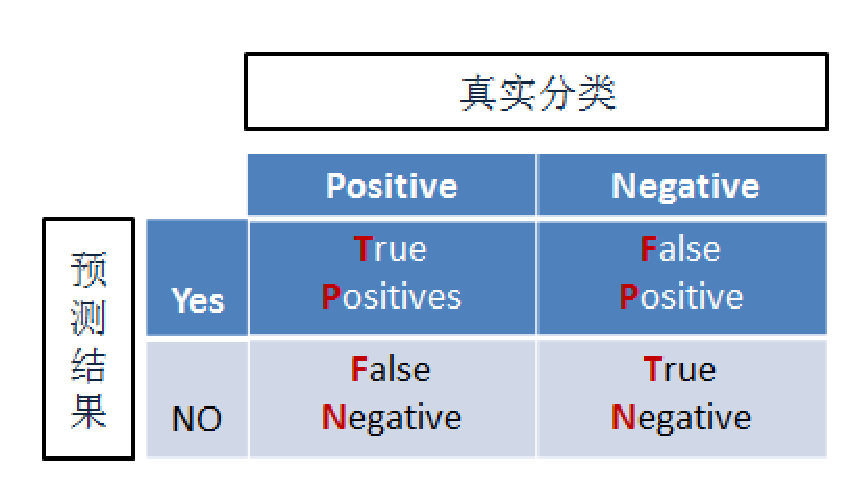
\includegraphics[width=0.5\textwidth, height = 5cm]{figures/labelandpredict.eps}
  \caption{真实标记与预测结果}\label{fig:labelandpredict}
\end{figure}
图\ref{fig:labelandpredict}构成一个分类器可信度的混淆矩阵(Confusion Matrix),以医学诊断\footnote{一般来说,阳性表示疾病或体内生理的变化有一定的结果,
阴性则基本上否定或排除某种病变的可能性}为例,其中的阳性(Positive)是“有病”,阴性(Negative)是“无病”,则False Positve是“假阳性”,将实际“无病
(Negative)”的人诊断为“有病(True)”,也称“误诊率”,属于“第I类错误”。False Negative是“假阴性”,将实际“有病(Positive)”的人诊断为“无病(False)”,也称“漏诊率”,属于“第II类错误”。统计学家认为犯第I类错误的代价高于犯第II类错误,实际上在不同的治疗阶段,两类错误的代价是不同的。

根据Precision与Recall的定义,结合图\ref{fig:labelandpredict},我们有:
\begin{equation}
  \begin{array}{l}
    \text{P} = \frac{\text{TP}}{\text{TP + FP}} \\
    \text{R} = \frac{\text{TP}}{\text{TP + FN}}
  \end{array}
\end{equation}

另外,根据预测与真实分类之间的一致性,还可以定义准确率(Accurate)、真阳性比率(True Positive Rate,TPR)、假阳性比率(False Positive Rate,FPR):
\begin{equation}
  \begin{array}{rcl}
    \text{Accurate} &=& \frac{\text{TP + TN}}{\text{TP + FP + TN + FN}} \\
    \text{TPR} &=& \frac{\text{TP}}{\text{TP + FN}} \\
    \text{FPR} &=& \frac{\text{FP}}{\text{FP + TN}} = 1 - \frac{\text{TN}}{\text{FP + TN}}
  \end{array}
\end{equation}

在20世纪50年代,英国Cranfield大学首先提出一套信息检索评价系统(简称Cranfield评价体系),由查询样本集、正确结果集和评价指标构成,并由此确立了“评价”在信息检索研究中的重要地位。Cranfield评价体系使用的两个评价指标是查准率和查全率,反映了标准检索系统的具备的两个基本能力:过滤不相关文档的能力,检索到所有相关文档的能力。查准率与查全率实际上是相互制约的,一般而言,查准率越高,则查全率下降,反之亦反。以查全率作为横轴,以查准率作为纵轴,二者的互斥关系可以使用Precison-Recall曲线(简称PR-Curve)\cite{davis2006relationship}描述,见图\ref{fig:prcurve}。

\begin{figure}[ht]
    \begin{minipage}[t]{0.49\linewidth}
        \centering
        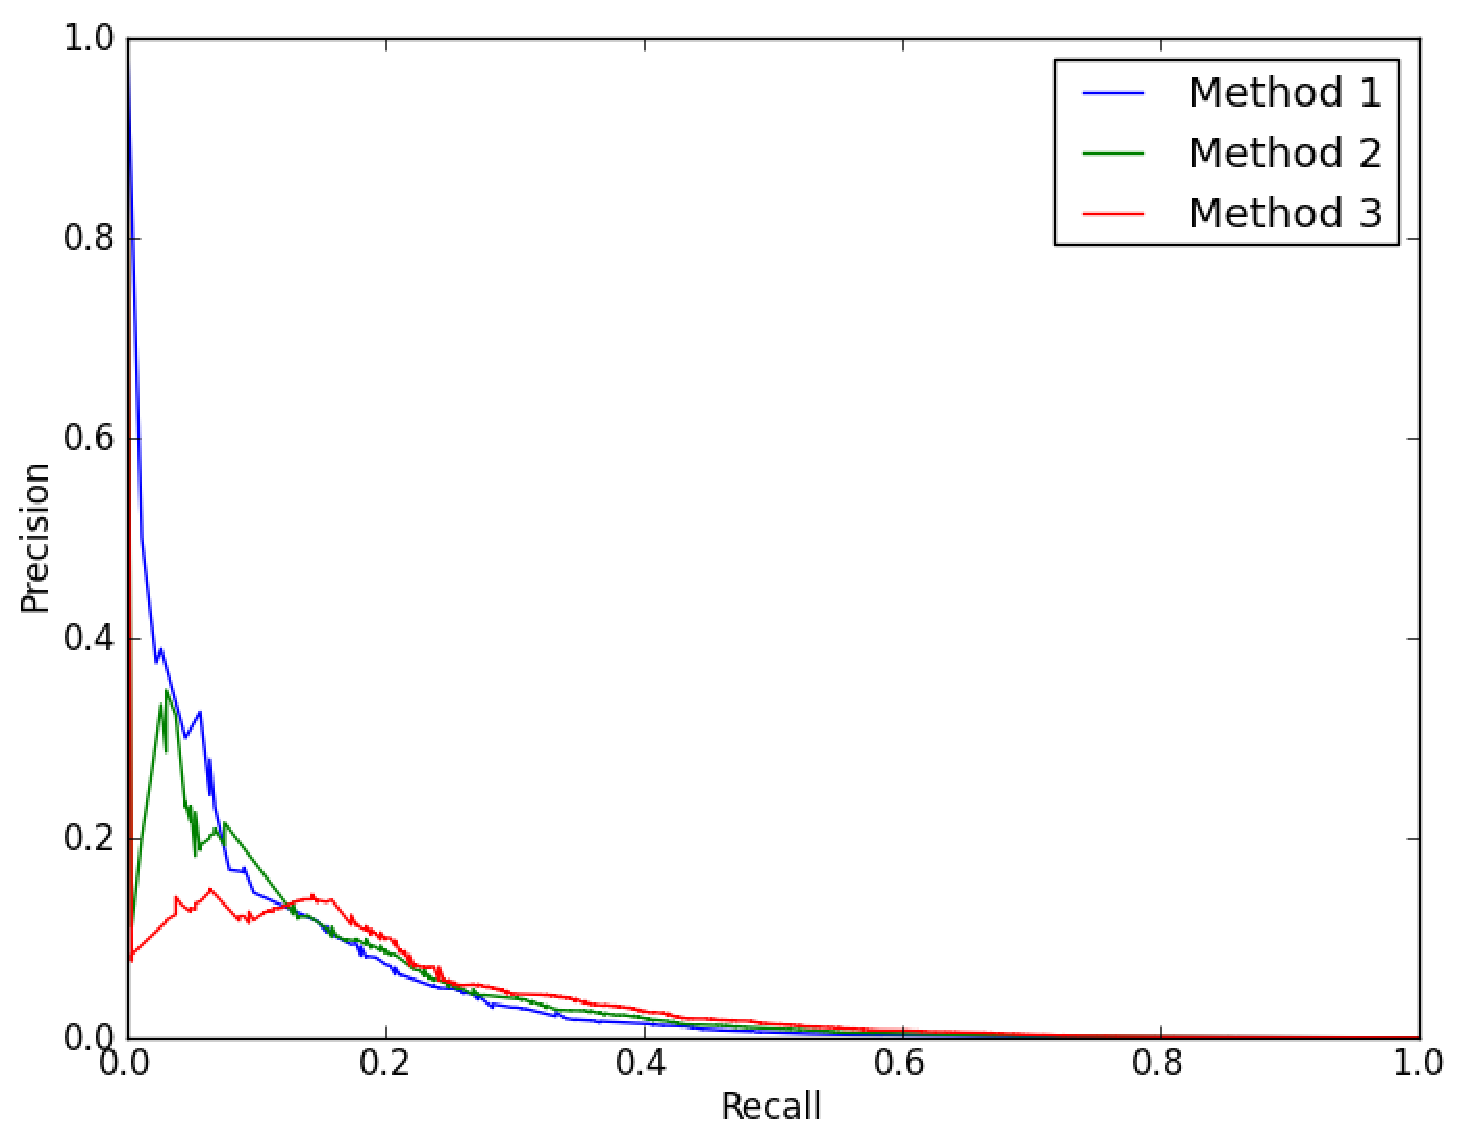
\includegraphics[width=0.95\textwidth, height = 8cm]{figures/prcurve.eps}
        \caption{PR曲线}\label{fig:prcurve}
    \end{minipage}
    \begin{minipage}[t]{0.49\linewidth}
        \centering
        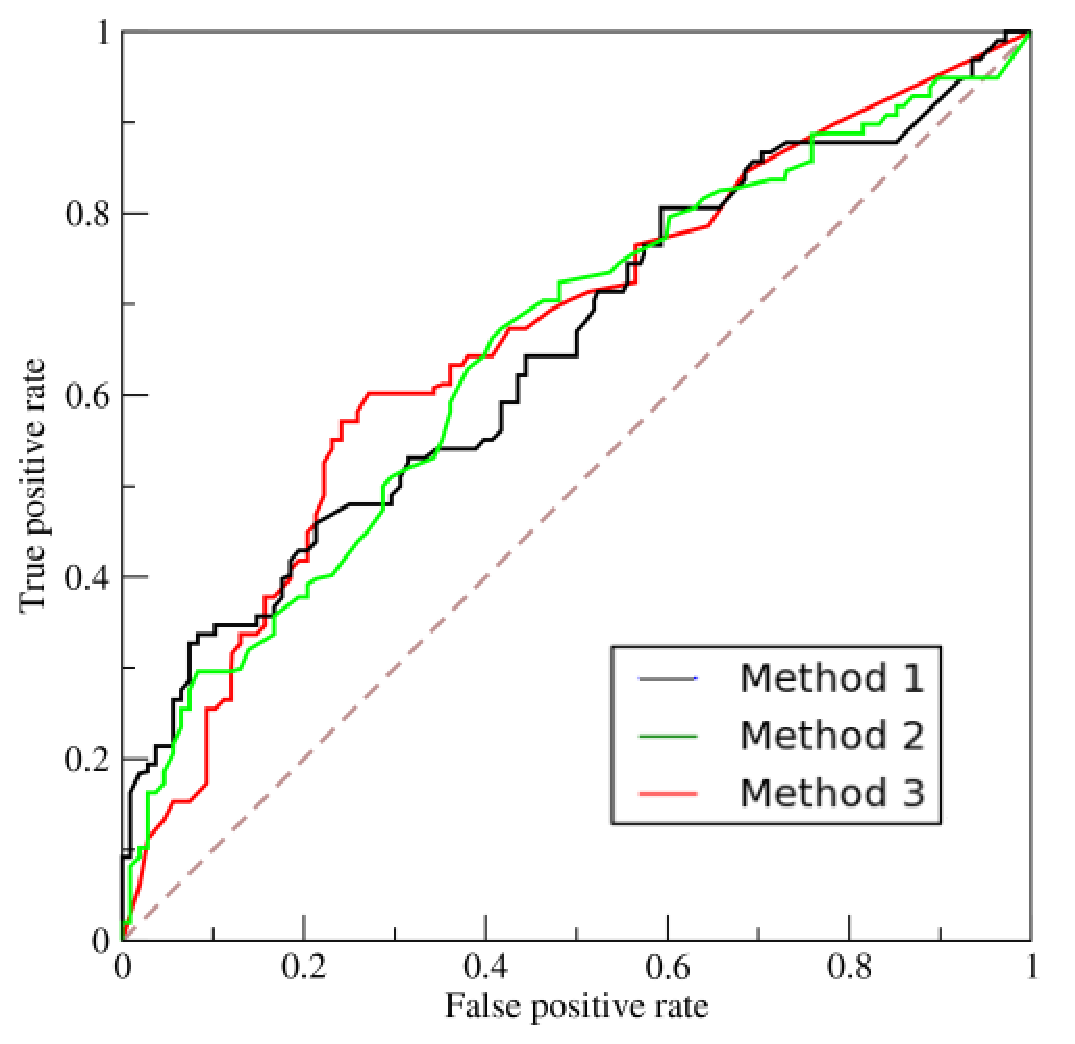
\includegraphics[width = 0.95\textwidth, height = 8cm]{figures/roccurve.eps}
        \caption{ROC曲线}\label{fig:roccurve}
    \end{minipage}
\end{figure}

为了融合查准率与查全率两种指标,学术界提出了如下定义的F度量(F-Measure):
\begin{equation}\label{eq:fmeasure}
  \text{F} = \frac{1}{\lambda\frac{1}{\text{P}} + (1-\lambda)\frac{1}{\text{R}}}
\end{equation}
其中,P表示查准率,R表示查全率,$\lambda \in (0,1)$平衡两个指标的作用,通常取$\lambda=0.5$,则有:
\begin{equation}\label{eq:0.5fmeasure}
  \text{F} = \frac{2\text{PR}}{\text{P+R}}
\end{equation}
此时,又称F度量为$F_1$度量。

ROC曲线(受试者工作特征——Receiver Operator Characteristic)源于信号检测理论,并广泛应用于机器学习和数据挖掘领域,是模型选择与评估的一个重要工具。在二元分类问题中,研究人员使用ROC曲线形象地刻画分类模型的假阳性率(横轴)与真阳性率(纵轴)之间的关系。对于完全随机分类模型,其ROC 曲线是连接原点与$(1,1)$ 的45°角平分线,任何优于随机分类的模型,其ROC曲线都位于45°平分线上方(见图\ref{fig:roccurve})
\footnote{在讨论ROC与PR曲线时,可能涉及到凸壳(Convex Hull),也称凸包(Convex Envelop)的概念,简单而言,在实数向量空间$V$中,对于给定集合$X$的凸包$S$ 是指$V$中所有包含$X$的凸集$K$的交:\[S = \bigcup\limits_{X\subseteq K \subseteq V} K,\]如果$X$是有限的,则$X$的凸包可以由$X$内所有点$(x_1,\ldots,x_n)$ 线性组合来构造:\[S = \{\sum\limits_{i = 1}^n \alpha_i x_i \mid x_i\in X, \sum\limits_{i = 1}^n \alpha_i = 1, \alpha_i \in [0,1]\}\]}。
ROC曲线下方面积AUC\cite{bradley1997use}可用来衡量模型预测的准确性,指标范围在$[0,1]$之间,有趣的是AUC同Wilcoxon-Mann-Whitney统计量是等价的~\cite{hanely1982meaning},可用于衡量分类模型的排名性能。

\subsection{平均精度均值}
根据精度的定义,可以定义平均精度(Average Precision):
\begin{equation}\label{eq:ap}
    \text{AP}=\frac{1}{n_1} \sum_{k=1}^{n}{I(y_{\pi^{-1}(k)}=1)\text{P@k}}
\end{equation}
其中,$n$是与检索词关联的文档数目,$n_1$表示相关文档的数目,在PR曲线中,平均精度近似地等于曲线下方面积所占比例。

平均精度均值(Mean Average Precision,MAP)是指所有检索词上的AP的平均值,即
\begin{equation}\label{eq:map}
    \text{MAP} = \frac{1}{|Q|}\sum_{q\in Q}{\text{AP}(q)}
\end{equation}

\subsection{折损累积增益}
折损累积增益(Discounted Cumulative Gain,DCG)是评价排名质量的一种标准指标,常用于度量搜索排名算法的精度,在信息检索领域有广泛使用。它不局限于评价仅含有相关、不相关两种评分相关等级的排名问题,对于包含多个评分相关等级的排名问题同样适用。给定一个排名列表,折损累积增益根据文档在排名列表中的位置信息计算其有用性或称增益量,从排名列表的顶部到底部累积各个位置的增益量,并以各自的位置信息进行折损。一般地,如果相关性越高则越有用,相应地在排名列表中的位置越靠前,则折损累积增益的值就越高。在评价排序模型的质量时,如果折损累积增益的值越大,则认为排序模型性能越高。

在折损累积增益诞生之前,常使用一种称为\textbf{累积增益}的指标,它只是将对应位置以后所有对象的评分相关等级机械相加,没有将位置信息计入增益量。对于给定的排名列表$\pi$,在位置$k$处的累积增益定义如下:
\begin{equation}
    \text{CG@k} = \sum\limits_{i=1}^k y_{\pi^{-1}(i)}
\end{equation}
其中,$\pi^{-1}(i)$表示在排名列表中排在位置$i$的对象,其相关等级用$y_{\pi^{-1}(i)}$表示。在累积增益的计算过程中,如果调换排名在$[1,k]$范围内任意两个对象的位置,无论是将相关的对象位置往后挪,还是将不相关对象的位置向前移,都不会影响累积增益量。折损累积增益克服了累计增益的这一缺陷,对于不同位置的增益设置不同的折损:位置靠前的对象折损越小,有用性更高。对于位置$k$处的折损累积增益定义如下:
\begin{equation}
    \text{DCG@k} = y_{\pi^{-1}(1)} + \sum\limits_{i=2}^k \frac{y_{\pi^{-1}(i)}}{\log i}
\end{equation}
或者
\begin{equation}
    \text{DCG@k} = \sum\limits_{i=1}^k \frac{2^{y_{\pi^{-1}(i)}}-1}{\log (i+1)}
\end{equation}
其中,公式加和项分数的分子部分表示\textbf{增益},分母部分表示\textbf{折损}。通过选择不同截断位置(Cut-off),折损累积增益可以评价不同位置上的排名质量。

在网络搜索应用中,由于不同搜索引擎所使用的排名算法不同,对于同一个检索词,每个系统返回的搜索结果数量也不相同。为方便比较不同搜索引擎、不同排名算法,需要对折损累积增益在检索词上做标准化处理。假设对于每一个检索词,都存在一个真实的排名列表,如果某个排序模型的预测排名与真实排名完全一致,我们称之为理想排名模型,相应排名结果称为\textbf{理想排名},而根据理想排名列表计算的折损累积增益也称\textbf{理想累积增益}。理想累积增益在位置$k$截断值记作$Z_k$,利用它标准化折损累积增益就得到\textbf{标准累积增益}:
\begin{equation}
    \text{NDCG@k} = \frac{\text{DCG@k}}{Z_k}
\end{equation}
取值范围在$[0,1]$,它是评价排序模型或算法质量最常用的一种标准指标。

\subsection{倒数排名均值}
倒数排名均值(Mean Reciprocal Rank,MRR)是一种衡量两个级别的排名质量的度量方式,是倒数排名(Reciprocal Rank, RR)在检索词集合$Q$上的平均值。倒数排名是指对于某个检索词,相关文档最好的排名,即$\mathrm{RR}=r^{-1}$,$r$表示与检索词相关的文档最好的排名。比如,某个检索词的相关文档只有2个,其中一个排在第2位,另一个排在第10 位,那么其倒数排名为$2^{-1}$。对所有检索词的倒数排名取均值,就是平均倒数排名:
\begin{equation}\label{eq:mrr}
    \text{MRR}=\frac{1}{|Q|}\sum_{q\in Q}{\frac{1}{r_q}}
\end{equation}

\subsection{倒数排名期望}
倒数排名期望(Expected Reciprocal Rank,ERR)由Chapelle等人\cite{chapelle2009expected}提出,通过用户对搜索结果满意程度的统计模型分析,ERR表现优于DCG度量。

假设位置$j$的文档让用户满意的概率为$R_j$,则用户在位置$r$找到心仪的文档并停止浏览和查找的概率为:
\[
    \prod_{j=1}^{r-1}{(1-R_j)R_r}
\]
一般地,$R_j$可以使用对应位置文档的等级表示:
\[
    R_j=\frac{2^{y_j}-1}{2^{y_{\max}}}
\]

ERR可以定义为下式:
\begin{equation}\label{eq:err}
    \text{ERR} = \sum_{r=1}^{n} \frac{1}{r}\prod_{j=1}^{r-1}{(1-R_j)}R_r
\end{equation}
其中$n$表示待排名的文档数目;$y_i$表示排在$i$的文档等级;$y_{\max}$表示文档的最高等级。

\subsection{pFound}
pFound由Gulin等人\cite{gulin2009pfound}提出,Yandex从2007年就开始用它来评估搜索效果。与ERR类似,pFound也是一种衡量用户满意程度的概率模型。
\begin{equation}\label{eq:pfound}
    \text{pFound} = \sum_{r=1}^{n}{\prod_{j=1}^{r-1}{(1-b)(1-R_j)R_r}} = \sum_{r=1}^{n}{(1-b)^{r-1}}\prod_{j=1}^{r-1}{(1-R_j)R_r}
\end{equation}
$R_j$与ERR中的含义相同,表示用户在$j$处找到满意文档的概率;$b$表示在各个位置停止查找的概率,默认取值0.15。

ERR和pFound都基于相同的假设:(i)用户从上到下逐个浏览搜索结果页面;(ii)用户逐个点击搜索结果,直到找到目标文档或者没有找到而放弃搜索。

\subsection{胜者全拿}
胜者全拿(Winner Takes All,WTA)是一种两级别度量,对于某个检索词,如果排名最前的文档与之相关,则WTA损失为0,否则为1。

\section{信息度量}
信息论是运用概率论与数理统计的方法研究信息、信息熵、通信系统、数据传输、密码学、数据压缩等问题的应用数学学科。Shannon和Weaver于1948年10月发表在《贝尔系统技术学报》的论文\textbf{通信的数学原理}\cite{shannon1948mathematical},可以视作是现代信息论研究的开端。Claude Shannon由于在信息理论中的突出贡献被后人尊称为“信息论之父”。

\begin{figure}[htbp]
\begin{minipage}[h]{0.33\linewidth}
\centering
  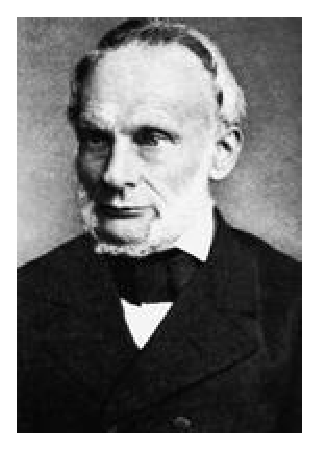
\includegraphics[width=0.9\textwidth, height=7cm]{figures/scientists/RudolfClausius.eps}
  \label{fig:RudolfClausius}
\end{minipage}
\begin{minipage}[h]{0.33\linewidth}
\centering
  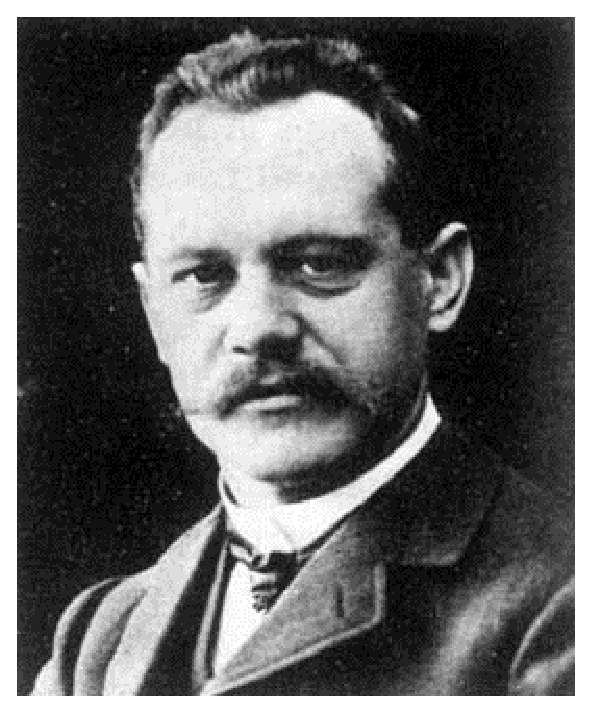
\includegraphics[width=0.9\textwidth, height=7cm]{figures/scientists/LudwigBoltzmann.eps}
  \label{fig:LudwigBoltzmann}
\end{minipage}
\begin{minipage}[h]{0.33\linewidth}
\centering
  \includegraphics[width=0.9\textwidth, height=7cm]{figures/scientists/claudeshannon.eps}
  \label{fig:claudeshannon}
\end{minipage}
\caption{Left:Rudolf Clausius (1822 - 1888), Middle:Ludwig Boltzmann (1844 - 1906), Right:Claude Shannon (1916 - 2001)}
\end{figure}

信息论将信息的传递作为一种统计现象来考虑,给出了估算通信信道容量的方法。信息传输和信息压缩是信息论研究中的两大领域,二者又通过信道编码定理、信源-信道隔离定理相互联系。信源编码和信道编码是信息论的基本研究课题。

\subsection{熵}
19世纪60年代,德国物理学家Rudolf Clausius在研究实际热机中发现,实际热机工作时会产生“无法使用”的热量(如摩擦产生的热量),并首次提出“熵
(Entropy)”的概念,用来描述能量的耗散。19世纪70 年代,Ludwig Boltzmann在分析系统中微观粒子的统计行为时给出熵的统计学定义,并证明这种统计学意义上的熵与Cluasius给出的热力学熵是等价的,仅仅相差一个常数项(Boltzmann常数)。根据熵的统计学定义,热力学第二定律说明一个孤立系统倾向于混乱程度增加(即“熵增”)。

受此启发,Shannon和Weaver在\cite{shannon1948mathematical} 中提出信息熵(Information Entropy,简称“熵”)的概念,并证明熵与信息的不确定性存在等价关系,信息熵越大,意味着不确定性越大,从而事件所包含的信息量越大。

离散随机变量$X=\{x_1,\ldots,x_n\}$的熵用于度量隐含于变量$X$的值的不确定性程度,如果令$p(x)$表示$X=x$的概率,那么变量$X$的熵定义为:
\begin{equation}\label{eq:entropy}
  H(X) = E_X[I(x)] = -\sum_{x\in X}{p(x)\log p(x)}
\end{equation}
其中,$I(x)$表示单个信息的熵分布,有时称作\textbf{自信息}(Self Information),$E_X$表示期望。计算中使用的对数基底如果是2,熵的单位就是比特(bit),在用符号表达信息时,熵用来量化单个字符可以存储或传输的平均比特数。

如果随机变量$X$是连续的,则熵可以使用积分计算
\begin{equation}\label{eq:continualentropy}
  H(X) = -\int_x{p(x)\log p(x)}dx.
\end{equation}
根据连续随机变量$X$熵的定义,我们可以计算常见连续分布的熵,比如$X\sim N(\mu,\sigma^2)$,则其连续熵
\[
\begin{array}{lcl}
    H(X) &=& -\int_{-\infty}^{+\infty} \frac{1}{\sqrt{2\pi}\sigma} \exp\{-\frac{(x-\mu)^2}{2\sigma^2}\} \big[-\frac{(x-\mu)^2}{2\sigma^2} - \log \big(\sqrt{2\pi}\sigma\big)\big]dx\\
    &=&\log \big(\sqrt{2\pi}\sigma\big) \int_{-\infty}^{+\infty} \frac{1}{\sqrt{2\pi}\sigma} \exp\{-\frac{(x-\mu)^2}{2\sigma^2}\} dx + \frac{1}{2\sigma^2} \int_{-\infty}^{+\infty}(x-\mu)^2 \frac{1}{\sqrt{2\pi}\sigma} \exp\{-\frac{(x-\mu)^2}{2\sigma^2}\} dx\\
    &=& \frac{1}{2} \big[1 + \log(2\pi \sigma^2)\big],
\end{array}
\]
由此可以看出,服从正态分布的变量,其熵的大小只与方差有关,方差相同则对应的熵也相等,方差越大熵值越大。

\begin{theorem}
对于随机变量$X$,$H(X)\ge 0$,当且仅当随机变量服从均匀分布时,$H(X)$最大。对于离散变量$X$,如果它的可能取值为有限集合$\{x_1,\ldots,x_n\}$,则有$H(X) \le \log n$,当且仅当$p(x_i)=\frac{1}{n}$时,等式成立。
\end{theorem}

\subsection{联合熵}
如果将两个离散随机变量$X$和$Y$简单联合,构成新的联合随机变量$(X,Y)$,则新的联合随机变量的熵(Joint Entropy)定义为:
\begin{equation}\label{eq:jointentropy}
  H(X,Y) = E_{X,Y}[I(x,y)] = -\sum_{x,y}{p(x,y)\log p(x,y)}
\end{equation}

如果事件$X$和$Y$是相互独立的,则$p(x,y)=p(x)p(y)$,那么
\[
  H(X,Y) = -\sum_{x,y}{p(x)p(y)\log(p(x)p(y))}= -\sum\limits_{x} p(x)\log p(x)-\sum\limits_y p(y)\log p(y)=H(X) + H(Y)
\]
\subsection{交叉熵}
假设随机变量$X$的概率密度函数为$P(X)$,许多情况下$P(X)$是未知的,人们通常使用统计的手段得到$P(X)$的近似分布$Q(x)$,则随机变量$X$的交叉熵(Cross Entropy)定义为:
\begin{equation}\label{eq:crossentropy}
  H(P(X),Q(X)) = -\sum_{x\in X}{P(x)\log Q(x)}
\end{equation}

如果将交叉熵引入计算机语言学,可以处理机器翻译的歧义问题。采用语句的真实语义作为交叉熵的训练集的先验信息,将机器翻译的语义作为测试集后验信息,使用两者的交叉熵指导对歧义的辨识和消除。
\subsection{条件熵}
设有随机变量$X,Y$,其联合概率分布为
\[
    p(x,y) = P(X=x, Y = y)
\]
条件熵(Conditional Entropy)$H(X|Y)$表示已知随机变量$Y$的条件下,随机变量$X$的不确定性,并做如下定义:
\begin{equation}\label{eq:conditionalentropy}
    \begin{array}{lll}
        H(X\mid Y) & = & E_Y[H(X|Y=y)] \\
         & = & \sum\limits_y p(y) H(X|Y=y)\\
         & = & -\sum\limits_y p(y)\sum\limits_x{p(x|y)\log p(x|y)} \\
         & = & -\sum\limits_{x,y} p(x,y)\log\frac{p(x,y)}{p(y)} \\
         & = & H(X,Y) - H(Y)
    \end{array}
\end{equation}
$H(X|Y)$表示随机变量$Y$给定条件下,$X$的条件概率分布熵在$Y$上的数学期望。

\subsection{KL散度}
KL散度(Kullback–Leibler Divergence)\cite{kullback1951information,kullback2012information},又称相对熵(Relative Entropy)或信息散度(Information Divergence)是度量两分布(真实概率分布与任意概率分布)之间距离的一种方式。假设存在某真实分布$p(X)$ 及任意一个分布$q(X)$,则两分布之间的KL散度定义为:
\begin{equation}\label{eq:relativeentropy}
  D_{KL}(p(X)\|q(X)) = \sum_{x\in X}{p(x)\log\frac{p(x)}{q(x)}}
\end{equation}
根据交叉熵的定义可知:
\begin{equation}
    D_{KL}(p(X)\|q(X)) = \sum_{x\in X}{p(x)\log\frac{p(x)}{q(x)}} = -\sum_{x\in X}{p(x)\log q(x)} - H(X) = H(p(X),q(X)) - H(X)
\end{equation}

\begin{lemma}
对任意两个分布$p(X)$与$q(X)$,都有$D_{KL}(p(X)\|q(X))\ge 0$,当且仅当$p(X)=q(X)$时,$D_{KL}(p(X)\|q(X))= 0$。
\end{lemma}
\begin{lemma}[Pythagorean性质]
如果$p\in P$,$q\in Q$,$\hat p\in P\cap Q$,则有
\[
    D_{KL}(p(X)\|q(X))=D_{KL}(p(X)\|\hat p(X)) + D_{KL}(\hat p(X)\|q(X)).
\]
\end{lemma}

\begin{theorem}[最大熵解]
如果$\hat p\in P\cap Q$,则解
\begin{equation}
    \hat p = \argmax\limits_{p} H(p)
\end{equation}
存在且唯一。
\end{theorem}

\begin{theorem}[最大似然解]
如果$\hat p\in P\cap Q$,则解
\begin{equation}
    \hat p = \argmax\limits_{q} L(q)
\end{equation}
存在且唯一。
\end{theorem}

\begin{theorem}[对偶定理]
存在唯一的分布$\hat p$,满足
\begin{equation}
    \hat p = \argmax\limits_{p} H(p) = \argmax\limits_{q} L(q) \in P\cap Q.
\end{equation}
\end{theorem}
根据对偶定理可知,最大熵解可以写作对数线性形式,解出最大似然解就给出了最大熵解。

\begin{figure}[htbp]
\begin{minipage}[h]{0.49\linewidth}
\centering
  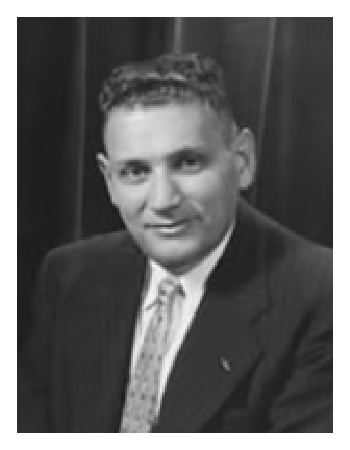
\includegraphics[width=0.95\textwidth, height=9cm]{figures/scientists/SolomonKullback.eps}
  \caption{Solomon Kullback (1907 - 1994)}\label{fig:SolomonKullback}
\end{minipage}
\begin{minipage}[h]{0.49\linewidth}
\centering
  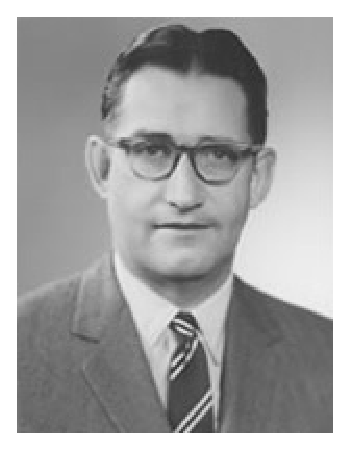
\includegraphics[width=0.95\textwidth, height=9cm]{figures/scientists/RichardLeibler.eps}
  \caption{Richard Leibler (1904 - 2003)}\label{fig:RichardLeibler}
\end{minipage}
\end{figure}

在数据压缩应用中,假设数据服从分布$q(X)$并执行压缩,而数据真实分布为$p(X)$,则KL-散度表示相对理想情况,压缩数据需要的平均额外的支出(比特)。
从信息论的角度来看,如果随机变量的真实分布为$p(X)$,然而人们却错误地使用概率密度函数$q(X)$,则KL散度刻画了由于使用错误的分布密度函数而导致信息量的增加。

\subsection{互信息}
互信息(Mutual Information)表示通过观察一个随机变量,从另外一个随机变量中获取的信息量,它是通信理论中的一个重要指标,常用于最大化发送信号和接收信号间共享的信息量。随机变量$X$相对$Y$的互信息定义为:
\begin{equation}\label{eq:mutualinfo}
  I(X;Y) = \sum_{X,Y}{p(x,y)\log\frac{p(x,y)}{p(x)p(y)}} = H(X) - H(X|Y) = H(X) + H(Y) - H(X,Y)
\end{equation}
由此可知,在知道$Y$的情况下为$X$编码,相比不知道$Y$的情况下,可以节省$I(X;Y)$个比特。由定义可知,互信息$I(X;Y)$是对称的。如果随机变量$X$和$Y$是相互独立的,由$H(X,Y)=H(X) + H(Y)$可知$I(X;Y)=0$。

根据等式
\[
 D_{KL}(p(X|Y=y)\| p(X)) = \sum_{x\in X}{p(x|y)\log\frac{p(x|y)}{p(x)}}=\sum_{x\in X}{p(x|y)\log\frac{p(x,y)}{p(x)p(y)}}
\]
可以使用KL-Divergence表示互信息:
\[
    I(X;Y) = \sum_{x\in X}{p(x|y)p(y)\log\frac{p(x,y)}{p(x)p(y)}} = E_{p(y)}[D_{KL}(p(X|Y=y)\|p(X))]
\]
联合熵、条件熵、互信息三者之间的关系可以通过图\ref{fig:entropy}形象表示。
\begin{figure}[ht]
  \centering
  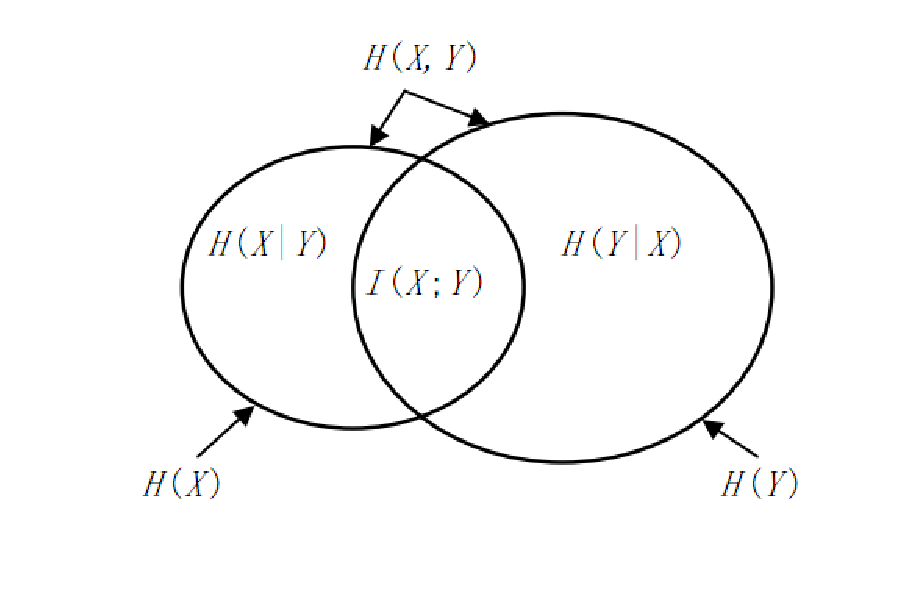
\includegraphics[width=0.6\textwidth]{figures/entropy.eps}
  \caption{联合熵、条件熵、互信息三者之间的关系}\label{fig:entropy}
\end{figure}

\subsection{詹森--香农散度}
詹森--香农散度(Jensen--Shannon Divergence),也称信息半径(Information Radius,IRad),在统计学中,常用作衡量两个概率分布的相似度。JS散度建立在KL散度之上,但又不同于KL散度:JS散度是对称的。它最初为Dagan Ido等人用于计算单词的相似性\cite{dagan1999similarity},现在已经成为生物信息学重要的度量工具。

对于两个概率分布$P$与$Q$,它们的JS散度定义为两个KL散度的均值:
\begin{equation}
  D_{JS}(P\| Q) = \frac{1}{2}(D_{KL}(P\| M) + D_{KL}(Q\| M))
\end{equation}
其中,$M = (P + Q)/2$表示$P,Q$的混合概率分布。根据定义可知$D_{JS} \in [0,1]$:
\begin{equation}
\begin{array}{ll}
  D_{JS}(P\| Q) & = \frac{1}{2}(\sum P\log{\frac{P}{M}} + \sum Q\log{\frac{Q}{M}})\\
   & = H(M) - \frac{1}{2}H(P) - \frac{1}{2}H(Q)
\end{array}
\end{equation}

假设$X$是服从混合分布$M$的随机变量,$Z$表示二元示性变量(Binary Indicator Variable),如果$X$服从$P$时,则$Z=1$,如果$X$服从$Q$时,则$Z=0$。变量$X$与$Z$的互信息
\begin{equation}
\begin{array}{ll}
  H(X;Z) & = H(X) - H(X|Z)\\
   & = \sum M\log M - \prob(Z = 0) H(X|0) - \prob(Z = 1)H(X|1)\\
   & = H(M) - \frac{1}{2}H(P) - \frac{1}{2}H(Q)
\end{array}
\end{equation}
与概率分布$P$和$Q$的JS散度等价。

\subsubsection{最小编码长度}
哈夫曼编码是由戴维·哈夫曼David A. Huffman于1952年提出,属于一种典型的变长编码(Variable Length Coding, VLC)方式,基于“高频字母短编码,低频字母长编码”的原则实现最优编码,主要用于文本文件的无损压缩(Lossless Compression)。
\begin{figure}[t]
  \centering
  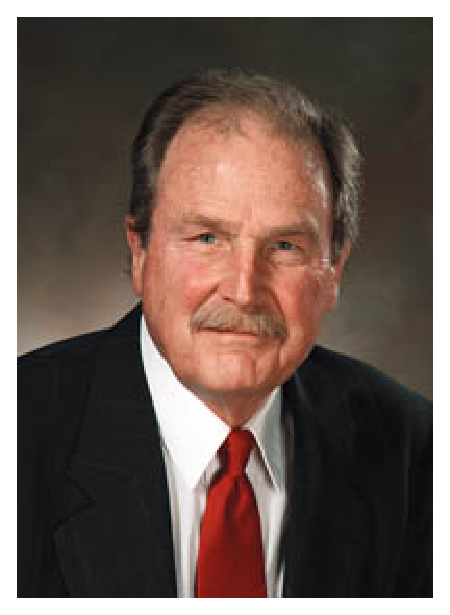
\includegraphics[width=0.3\textwidth, height = 7cm]{figures/scientists/DavidHuffman.eps}\\
  \caption{David Albert Huffman (1925 - 1999)}\label{fig:DavidHuffman}
\end{figure}

哈夫曼编码的目标是寻找最有效率的编码方式,使得平均编码长度最短。可以证明哈夫曼编码是满足最小信息熵的编码。
\subsubsection{Fano不等式}
